Sendo assim, seja pela convergência do grau de utilização normal ao efetivo, seja pela presença de um corredor de estabilidade ou objetivos conflitantes das firmas, a instabilidade de Harrod é resolvida às custas da não replicação do fato estilizado reportado acima. Logo, a preservação das características dos modelos Kaleckianos canônicos impôs a hipótese pouco razoável de que o grau de utilização (efetivo ou normal) acomodará variações no nível de atividade e não a taxa de acumulação. Desse modo, o trecho de \textcite[p.~135]{skott_theoretical_2012} reproduzido abaixo é bastante ilustrativo:

\begin{citacao}
Mathematically it is not difficult to set up a model that generates Kaleckian results. The desired rate may adapt to the actual rate, and assuming
certain conditions with respect to adjustment speeds, we may get a model that
generalizes the canonical model; the key properties of the simple model are
retained but, because of the non-uniqueness of the stationary solution, path
dependence may be present. The behavioral story behind the equations does
not, however, seem plausible.
\end{citacao}

Por fim, a seção \ref{debate} retratou o debate entorno da convergência (ou não) do grau de utilização ao nível desejado no longo prazo. Verificou-se que as características dos modelos Kaleckianos tradicionais são preservadas se são adicionadas novas hipóteses ao modelo. Argumentou-se que a necessidade de tais modificações decorrem do não abandono da autonomia do investimento produtivo no longo prazo. Diante disso, a discussão centrou-se na endogeneidade do grau de utilização (seja ele efetivo ou desejado), relegando a um plano secundário uma questão igualmente relevante: quão induzido/autônomo é o investimento produtivo no longo prazo? Este é um dos temas do capítulo seguinte.


\begin{comment}
\begin{figure}
    \centering
\begin{venndiagram3sets}[labelA=,labelB=,labelC=,labelOnlyA = \(\gamma \neq 0\),labelOnlyB = \(Z > 0\),labelOnlyC = \(u \to u_n\)]

\fillANotB
\fillANotC
\fillOnlyB
\fillCNotB
\end{venndiagram3sets}
\caption{Caption}
\end{figure}


O diagrama de Venn abaixo ilustra esse raciocínio:


\begin{figure}[H]
    \centering
    \caption{Relação entre hipótese Keynesiana e instabilidade de Harrod}
    %\label{fig:my_label}
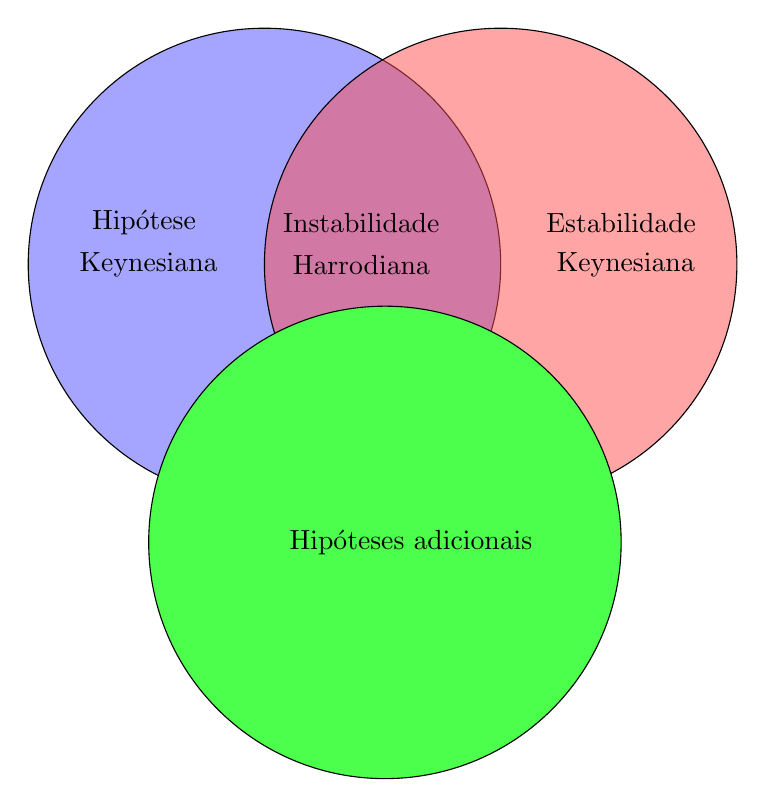
\begin{tikzpicture}
\def\radius{3cm}
\def\mycolorbox#1{\textcolor{#1}{\rule{2ex}{2ex}}}
\colorlet{colori}{blue!70}
\colorlet{colorii}{red!70}
\colorlet{coloriii}{green!70}

\coordinate (ceni);
\coordinate[xshift=\radius] (cenii);
\coordinate[yshift=-3.5\radius, xshift=1.5\radius] (ceniii);

\draw[fill=colori,fill opacity=0.5] (ceni) circle (\radius);
\draw[fill=colorii,fill opacity=0.5] (cenii) circle (\radius);
\draw[fill=coloriii,fill opacity=1] (ceniii) circle (\radius);


\node[yshift=.5\radius, xshift=-1.5\radius] at (ceni) {\text{Hipótese}};
\node[xshift=-1.5\radius] at (ceni) {\text{ Keynesiana}};
\node[yshift=.5\radius, xshift=1.5\radius] at (cenii) {\text{Estabilidade}};
\node[xshift=1.5\radius] at (cenii) {\text{ Keynesiana}};
\node[yshift=.5\radius, xshift=1.2\radius] at (ceni) {\text{Instabilidade}};
\node[xshift=1.2\radius] at (ceni) {\text{Harrodiana}};
\node[xshift=.3\radius] at (ceniii) {\text{Hipóteses adicionais}};
\end{tikzpicture}
\caption*{\textbf{Fonte:} Elaboração própria}
\end{figure}
\end{comment}

%DEJUAN: Retomada do supermultiplicador

%LINHAS DE PESQUISAS NECESSÁRIAS INDICADAS POR ALLAIN

%LAVOIE E FIEBGER: INVESTIMENTO RESIDENCIAL